% !TEX TS-program = XeLaTeX
% use the following command:
% all document files must be coded in UTF-8
\documentclass[english]{textolivre}
% build HTML with: make4ht -e build.lua -c textolivre.cfg -x -u article "fn-in,svg,pic-align"
\setotherlanguage{spanish}

\journalname{Texto Livre}
\thevolume{18}
%\thenumber{1} % old template
\theyear{2025}
\receiveddate{\DTMdisplaydate{2024}{12}{16}{-1}} % YYYY MM DD
\accepteddate{\DTMdisplaydate{2025}{2}{14}{-1}}
\publisheddate{\DTMdisplaydate{2025}{8}{04}{-1}}
\corrauthor{Carmen María Sánchez Morillas}
\articledoi{10.1590/1983-3652.2025.56537}
%\articleid{NNNN} % if the article ID is not the last 5 numbers of its DOI, provide it using \articleid{} commmand 
% list of available sesscions in the journal: articles, dossier, reports, essays, reviews, interviews, editorial
\articlesessionname{dossier}
\runningauthor{García Fernández, Jodar Jurado and Sánchez Morillas} 
%\editorname{Leonardo Araújo} % old template
\sectioneditorname{Hugo Heredia Ponce}
\layouteditorname{Saula Cecília}

\title{The teaching of Spanish as a foreign language and artificial intelligence: the beliefs of the student teachers at the University of Jaén}
\othertitle{Ensino de espanhol como língua estrangeira e inteligência artificial: crenças de professores em formação na Universidade de Jaén}

\author[1]{María García Fernández~\orcid{0000-0002-6437-2562}\thanks{Email: \href{mailto:magarcif@ujaen.es}{magarcif@ujaen.es}}}
\author[1]{Rocío Jodar Jurado~\orcid{0000-0002-3200-2241}\thanks{Email: \href{mailto:rjjurado@ujaen.es}{rjjurado@ujaen.es}}}
\author[1]{Carmen María Sánchez Morillas~\orcid{0000-0002-6622-212X}\thanks{Email: \href{mailto:cmsanche@ujaen.es}{cmsanche@ujaen.es}}}
\affil[1]{University of Jaén, Jaén, Spain.}


\addbibresource{article.bib}
% use biber instead of bibtex
% $ biber article

% used to create dummy text for the template file
\definecolor{dark-gray}{gray}{0.35} % color used to display dummy texts
\usepackage{lipsum}
\SetLipsumParListSurrounders{\colorlet{oldcolor}{.}\color{dark-gray}}{\color{oldcolor}}

% used here only to provide the XeLaTeX and BibTeX logos
\usepackage{hologo}

% if you use multirows in a table, include the multirow package
\usepackage{multirow}

% provides sidewaysfigure environment
\usepackage{rotating}

% CUSTOM EPIGRAPH - BEGIN 
%%% https://tex.stackexchange.com/questions/193178/specific-epigraph-style
\usepackage{epigraph}
\renewcommand\textflush{flushright}
\makeatletter
\newlength\epitextskip
\pretocmd{\@epitext}{\em}{}{}
\apptocmd{\@epitext}{\em}{}{}
\patchcmd{\epigraph}{\@epitext{#1}\\}{\@epitext{#1}\\[\epitextskip]}{}{}
\makeatother
\setlength\epigraphrule{0pt}
\setlength\epitextskip{0.5ex}
\setlength\epigraphwidth{.7\textwidth}
% CUSTOM EPIGRAPH - END

% to use IPA symbols in unicode add
%\usepackage{fontspec}
%\newfontfamily\ipafont{CMU Serif}
%\newcommand{\ipa}[1]{{\ipafont #1}}
% and in the text you may use the \ipa{...} command passing the symbols in unicode

% LANGUAGE - BEGIN
% ARABIC
% for languages that use special fonts, you must provide the typeface that will be used
% \setotherlanguage{arabic}
% \newfontfamily\arabicfont[Script=Arabic]{Amiri}
% \newfontfamily\arabicfontsf[Script=Arabic]{Amiri}
% \newfontfamily\arabicfonttt[Script=Arabic]{Amiri}
%
% in the article, to add arabic text use: \textlang{arabic}{ ... }
%
% RUSSIAN
% for russian text we also need to define fonts with support for Cyrillic script
% \usepackage{fontspec}
% \setotherlanguage{russian}
% \newfontfamily\cyrillicfont{Times New Roman}
% \newfontfamily\cyrillicfontsf{Times New Roman}[Script=Cyrillic]
% \newfontfamily\cyrillicfonttt{Times New Roman}[Script=Cyrillic]
%
% in the text use \begin{russian} ... \end{russian}
% LANGUAGE - END

% EMOJIS - BEGIN
% to use emoticons in your manuscript
% https://stackoverflow.com/questions/190145/how-to-insert-emoticons-in-latex/57076064
% using font Symbola, which has full support
% the font may be downloaded at:
% https://dn-works.com/ufas/
% add to preamble:
% \newfontfamily\Symbola{Symbola}
% in the text use:
% {\Symbola }
% EMOJIS - END

% LABEL REFERENCE TO DESCRIPTIVE LIST - BEGIN
% reference itens in a descriptive list using their labels instead of numbers
% insert the code below in the preambule:
%\makeatletter
%\let\orgdescriptionlabel\descriptionlabel
%\renewcommand*{\descriptionlabel}[1]{%
%  \let\orglabel\label
%  \let\label\@gobble
%  \phantomsection
%  \edef\@currentlabel{#1\unskip}%
%  \let\label\orglabel
%  \orgdescriptionlabel{#1}%
%}
%\makeatother
%
% in your document, use as illustraded here:
%\begin{description}
%  \item[first\label{itm1}] this is only an example;
%  % ...  add more items
%\end{description}
% LABEL REFERENCE TO DESCRIPTIVE LIST - END


% add line numbers for submission
%\usepackage{lineno}
%\linenumbers

\begin{document}
\maketitle

\begin{polyabstract}
\begin{abstract}
This study presents the findings of an action-research process conducted as part of the Teaching Innovation Project 'Culture and Inclusion' within the PIMED 2019-2023 plan of the University of Jaen. In particular, we have concentrated on the qualitative analysis of the data obtained regarding to the beliefs about the use of AI of teachers in SFL training through the discussion forum 'ICT and IA in the teaching of culture and ELE', which was developed from the optional subject Culture in the Classroom of Spanish as a Foreign Language, belonging to the specialisation module II on 'Teaching Spanish as a foreign language' of the Master's Degree in Spanish Language and Literature: research and applications of the University of Jaen. The focus group comprised 48 students. The main objective of this preliminary study is to ascertain the trainees' perceptions regarding the utilisation AI tools in the SLF classroom for the introduction of cultural elements, as well as their initiative and critical expression.

\keywords{Artificial Intelligence\sep Teacher training\sep Higher university education\sep Spanish as a Foreign Language (SFL)}
\end{abstract}

\begin{portuguese}
\begin{abstract}
Este estudo aborda a análise dos resultados derivados da aplicação de um processo de investigação-ação do Projeto de Inovação Docente ``Cultura e inclusão", no âmbito do plano PIMED 2019-2023 da Universidade de Jaén. Especificamente, nos concentramos na análise qualitativa dos dados obtidos sobre as crenças em torno do uso de IA de professores formadores de ELE por meio do fórum de debate ``TIC e IA no ensino da cultura e ELE", desenvolvido a partir da disciplina opcional Cultura na sala de Aula de Espanhol como Língua Estrangeira, pertencente a módulo II da especialização ``Ensino de espanhol como língua estrangeira" do Mestrado em Língua e Literatura Espanhola: Pesquisa e Aplicações da Universidade de Jaén. Este grupo de discussão foi composto por 48 alunos. Um dos principais objetivos deste primeiro estudo é conhecer a percepção dos alunos em formação relativamente à utilização da IA na sala de aula ELE na introdução de elementos culturais, bem como a iniciativa e expressão crítica destes futuros profissionais.

\keywords{Inteligência artificial\sep Professores em formação\sep Ensino superior universitário\sep Espanhol como Língua Estrangeira (ELE)}
\end{abstract}
\end{portuguese}
% if there is another abstract, insert it here using the same scheme
\end{polyabstract}

\section{Introduction}
The processes of language teaching and learning, as well as their corresponding methodologies, have undergone an accelerated evolution that has parallelled developments in other areas of knowledge since the implementation of Computer Assisted Language Teaching (CALL) and Mobile Assisted Language Teaching (MALL) \cite{gabarron-perez2020}. The advent and proliferation of social networks, in conjunction with the democratisation of technology precipitated by the advent of the pandemic, have collectively engendered an educational milieu that starkly contrasts with that of preceding decades. The advent of novel terminology such as Learning and Knowledge Technology (LKT) and Technologies for Empowerment and Participation (TEP), in conjunction with the emergence of Artificial Intelligence, has engendered the potential for the creation and implementation of learning environments that are characterized by a more intricate didactic approach, but more collaborative and active on the part of the students who use them \cite{gutierrez2022}.

In the field of foreign language teaching, the distinction made by \textcite{coello-munoz2023} between Information and Communication Technologies (ICT) for education and ICT in education appears to be pertinent. The former term refers to the development of tools and software specifically for language teaching, while the latter refers to the implementation of technologies and software specific to our society for educational purposes. Consequently, while computer applications such as Duolingo can be regarded as ICT tools for education, the utilisation of the possibilities offered by social networks in education is confined to the field of ICT in education. The selection of one or the other in the Spanish as a Foreign Language (SFL) classroom will depend, in our opinion, on several factors:
\begin{enumerate}[label=\alph*)]
    \item The presence or absence of adequate internet connectivity and the availability of computing devices, such as computers or mobile phones in the classroom. While ICT for educational purposes do permit off-line access through the use of CALL software in most cases, the utilization of ICT in education generally necessitates an internet connection and a connection to MALL.

    \item The content: many educational programmes specially designed for foreign language learning focus exclusively on the code, addressing aspects such as vocabulary, grammar and pronunciation. However, when it comes to developing communicative competence in a foreign language, it is generally more beneficial to employ ICT in education from a communicative approach \cite{badia-climent2024}, leveraging social networks, blogs, forums, streaming platforms and other similar tools.

    \item The interests and needs of learners.
\end{enumerate}


Regardless of the tools chosen, there is no doubt that ICT brings many advantages to the SFL classroom, such as (a) better access to a wide range of information and resources; (b) greater opportunities for communicative interaction; (c) better access to cultural content; (d) availability of virtual spaces for language immersion; (e) personalisation of the teaching and learning process according to the needs and interests of the learners; and (e) personalisation of the teaching and learning process according to the needs and interests of the learners \cite{intria2023, clementi2024}; (f) promotion of autonomy; (g) increased motivation; and, finally, (h) greater opportunities for innovation. To all this should be added the improvement of the ``flexibilidad de las clases y la administración del conocimiento [en] cuanto al desarrollo de las actividades dentro y fuera del aula [flexibility of teaching and knowledge management [in] the development of activities inside and outside the classroom]\footnote{A translation of all quotations in Spanish is provided in square brackets.}" \cite[p. 264]{moreno-padilla2019}. This has led to the emergence of blended learning models, in which virtual and face-to-face learning complement each other. The development of these models was stimulated after the Covid-19 pandemic \cite{bartolome2018, perez-garcia2021, roman2024, fabregat-barrios2024a}.

\section{Artificial intelligence in the teaching of Spanish as a Foreign Language}
In the field of teaching Spanish as a foreign language (SFL), the integration of artificial intelligence (AI) is modifying the manner in which information is accessed, and consequently impacting the process of acquiring a second or foreign language. In this regard, \textcite{portillo2024iaele} have observed that AI is not only revolutionising the field of technology, but is breaking into many sectors of society and changing the way we interact with technology and with each other.

The advent of novel AI-based models has given rise to a discourse surrounding the challenges and dangers of incorporating this technology into the foreign language classroom, particularly in the context of SFL \cite{chen2020, alam2021ai_education, ouyang2021review}. In this context, advances in AI systems, particularly Natural Language Processing (NLP), deep learning, and machine learning, have emerged as significant developments (see \textcite{gonzalez-gonzalez2023}. These technologies have the potential to personalise the foreign language acquisition process and automate assessment, thereby offering substantial benefits to educators and learners alike. In this regard, \textcite{ocana-fernandez2019} underscores the significance of digital literacy in effectively utilising these resources.

However, it is important to emphasise that the integration of AI in SFL teaching is not without its challenges. In this context, \textcite{canales2024} draws attention to a limitation that may affect the acquisition of Spanish due to the fact that it offers no explanation for the absence of accents. Furthermore, \textcite{sandoval2024} draws attention to the biases in the data provided by AI as a language model in the SFL classroom.

In language education, the integration of artificial intelligence has the potential to facilitate the creation of learning environments that necessitate ongoing updates to pedagogical expertise, underpinned by generative tools \cite{ayala2023}. In this regard, numerous language educators perceive a significant opportunity to enhance their practice by leveraging connections. Their future professional development with all the potentialities offered by generative teaching tools; these tools are being included in those teaching processes which, in turn, are based on the basic principles of neuroeducation \cite{rodriguez2024, mondejar2023}. In addition, teachers have indicated the value of exploring personalised language learning approaches, emphasising the importance of cultural content in this regard \cite{briceno-nunez2024, munoz-basols2024}.

In this context, teachers' beliefs about the use of AI and its positive use in the field of language teaching must be seen in the light of the first existing studies on the subject \cite{zamora2024}. Some of the most recent analyses on the use of AI tools highlight the growing pedagogical interest in the integration of chatbot, a tool that acts as a teacher, student or tutor in virtual environments \cite{moreno-padilla2019}, in conversational dialogue activities \cite{guano2023, lucana2023, de-almeida-ferreira2024} or the application of creative writing strategies mediated by OpenAI / GPT 3 \cite{vicente-yague-jara2023}.

On the other hand, an intermediate position asserts that, while AI offers a promising teaching environment, it is imperative to recognise the pivotal role of the teacher as a constant contributor in educational settings across various disciplines \cite{martin-marchante2022, rodriguez2024}. However, it is important to note that the integration of AI should not be regarded as a mere digital extension of ICT, as it has been demostrated \cite{toutain2023gestion}. Instead, it should be considered a fundamental disruptive change in the current educational paradigm. Such a transformation must mean that AI in language teaching must offer the opportunity for personalised but equitable learning for all learners; this view is of concern to many teachers in the sector \cite{munoz-basols2024, vera2023}.

In conclusion, scientific evidence suggests that ``es importante comprender los fundamentos de la IA y desarrollar nuestra alfabetización en IA para aprovechar su potencial en la mejora de los procesos de enseñanza-aprendizaje [it is important to understand the fundamentals of AI and to develop our AI literacy in order to take advantage of its potential to improve teaching-learning processes]" \cite[p. 114]{arroyo2024}. It is imperative to adopt a balanced approach that integrates technological innovation with pedagogical principles that align with the needs of students and the curriculum outlined in the \textit{Plan Curricular del Instituto Cervantes} \citeyear{cervantes2006}.

This paper sets out to explore the perceptions of 48 trainee teachers on the subject of Culture in the Spanish as a Foreign Language Classroom, as part of the Master's Degree in Spanish Language and Literature: Research and Applications at the University of Jaen. The focus of this study is on the utilisation of ICT and AI in the SFL classroom when introducing cultural elements. To this end, a qualitative analysis of the students' responses in the forum 'ICT and AI in the teaching of culture and SFL' will be conducted using a lexical recurrence program, ATLAS.TI, to ascertain and analyse their prevailing beliefs.This research is part of the Teaching Innovation Project 'Culture and Inclusion', which is part of the PIMED 2019-2023 plan of the University of Jaen.

In this respect, it should be noted that the work on the cultural dimension through new technologies and AI has already been the subject of study on numerous occasions \cite{rodriguezizquierdo2015competencias, leiva2022, briceno2024}. This link is particularly salient in the SFL classroom, as well as in the research with which we are concerned. In accordance with the \textit{Plan Curricular del Instituto Cervantes} \cite{cervantes2006}, three fundamental aspects must be addressed in terms of the development of intercultural competence: cultural references, sociocultural knowledge and behaviour, and intercultural skills and attitudes. The cultural references component encompasses a comprehensive set of general knowledge concerning Spanish-speaking countries, along with their most significant cultural products and creations (e.g., cinema, literature, music). The socio-cultural knowledge and behaviour component pertains to the living conditions and social conventions of the Spanish-speaking nations. Finally, with regard to intercultural skills and attitudes, the focus is on the configuration of a cultural identity, the processing and assimilation of cultural knowledge and socio-cultural behaviour, cultural interaction and, finally, cultural mediation.

\section{Objectives}
The present paper is grounded in the following research objectives:

\begin{enumerate}
    \item To conduct an analysis of students' beliefs in relation to the implementation of ICT and AI in the classroom, as well as their link with the formation of their teaching identity.
    \item To undertake an examination of the connections that students make between the content of SFL teaching, with a particular focus on those of a cultural nature, and the use of ICT and AI.
    \item To ascertain which ICT and AI tools learners use on a regular basis and for what purposes.
\end{enumerate}

\section{Methodology}
This study adopts a non-experimental, descriptive, qualitative methodology \cite{bourque2004, fowler2014}, based on the open-ended responses collected in the discussion forum ‘ICT and AI in the teaching of culture and SFL. These open-ended responses have been provided voluntarily by the students of the subject Culture in the Spanish as a Foreign Language Classroom of the Master's Degree in Spanish Language and Literature: Research and Applications at the University of Jaen. The work based on open-ended responses allows us to anonymously collect students' reflections, arguments and explanations about the teaching of SFL, paying special attention to cultural content and the use of ICT and AI.
 Finally, to ensure the accuracy of the English translation, the application \textcite{deepl2025} was utilised for cross-language checks.

\subsection{Participants}
A total of 48 students participated voluntarily in this research, comprising 44 women and 4 men, with ages ranging from 24 to 36. The vast majority of the participants (42 in total) hold a Bachelor's Degree in Spanish Philology, with 34 of these concurrently enrolled in a Master's Degree in Compulsory Secondary Education and Baccalaureate, Vocational Training and Language Teaching. The remaining students either have teaching degrees (two students) or have studied other philologies (four students).

The virtualisation of part of the master's programme, including this subject, also fosters the adaptability of the teaching and learning process. Consequently, a significant proportion of the student population (a total of 27 individuals) are employed as professionals seeking to enhance their understanding of research in the domain of language and literature. Additionally, approximately nine students aspire to progress their careers towards research and, thus, to enrol in doctoral programmes. Finally, approximately 12 students are unemployed or have not yet entered the labour market.

\subsection{Data collection instrument}
In line with the content presented in class, a discussion forum entitled ‘ICT and AI in the teaching of culture and SFL’ was opened, in which students were asked four questions closely related to the objectives of our research:

\begin{enumerate}
    \item At which levels of SFL teaching do you think the use of ICT and AI would be most appropriate?
    \item Do you think that the use of these resources in the classroom is beneficial for students or, on the contrary, counterproductive? And why?
    \item What content related to the teaching of Spanish as a foreign language would you address through the use of ICT or AI?
    \item What applications, software or programmes would you use to work on the content you have chosen?
\end{enumerate}

The data collection instrument utilised was, as previously stated, the discussion forum entitled 'ICT and AI in the teaching of culture and SFL'. This forum was developed through the University of Jaen's proprietary educational platform, PLATEA, which facilitates the incorporation of multiple discussion threads within a single forum. Consequently, the following discussion threads were established:

\begin{enumerate}[label=\alph*)]
    \item Educational levels of SFL teaching and implementation of ICT and AI:  is addressed in question a). In this particular thread, students were tasked with selecting appropriate levels for promoting the use of new technologies and artificial intelligence, and were expected to provide a concise justification. Additionally, students were given the opportunity to either refute or support their classmates' arguments.
    \item Benefits or disadvantages of using new technologies and AI in the SFL classroom: are outlined in question b). In this exercise, students were tasked with presenting arguments either in favour of or against the implementation of ICT and AI programmes in SFL teaching.
    \item SFL content, ICT and AI: related to question c). Following the selection of an educational level in the first thread, students were tasked with choosing a set of basic knowledge that, in their opinion, could be enhanced more effectively through the use of ICT and AI. They could select both linguistic knowledge related to language learning and cultural content.
    \item ICT and AI resources for classroom work: related to question d). Following the selection of the educational level and content, students were invited to select the ICT and AI resources they would use for their work in the SFL classroom. Many of the students who participated in this thread not only provided a list of resources, but also outlined some proposed activities in which they exemplified how they would implement these resources. This particular thread proved to be the most fruitful, as numerous learners contributed to refine their peers' proposals, offering a plethora of suggestions for enhancement.
\end{enumerate}

\subsection{Data analysis procedure}
The data were processed using a lexical recurrence analysis programme, ATLAS.ti, which enabled the quantitative analysis of the students' interventions in the forums. This procedure has previously been validated in a study by \textcite{fabregat-barrios2024b}.

The research has been developed according to the following phases:
\begin{enumerate}[label=\alph*)]
    \item The subject of Culture in the Spanish Classroom was taught and the forum was opened by the students.
    \item Student participation in the forums occurred during the course of the subject. Participation in each of the four threads was sequential, as the teachers had sequenced the beginning of each thread chronologically. Thus, the first discussion thread was on the use of ICT and AI in relation to the various levels of SFL teaching. It was not until this thread was considered by students and teachers to have been exhausted that the next one was opened. This sequencing enabled students to plan their interventions and afforded them time to reflect on the interventions of their peers.
    \item An initial qualitative analysis of the content of the responses \cite{caceres2023derecho} was conducted. In order to carry out this analysis and for the subsequent qualitative analysis, the teachers' interventions, which dealt with the discussion rules of the forum and the topic of each of the threads, were eliminated. These interventions would have generated noise in the subsequent quantitative analysis.
    \item Quantitative-lexical analysis was then conducted, with the results grouped in relation to the four threads described in the previous section.
    \item Delimitation of the productive base of words was then undertaken, followed by grouping by lexical families of the productive base. The results were then presented.
\end{enumerate}


\section{Results}
The quantitative analysis of the information was carried out with the support of the Atlas.ti 6.0 programme, which facilitates the processing and interpretation of the forum interventions through the study of the lexical recurrences recorded. In the present study, the productive base is made up of 7144 words out of a total of 12116 recorded in the forums. The programme permits the exclusion of words that lack semantic meaning and have only a grammatical function, thus allowing the delimitation of the productive base. In this way, words lacking semantic meaning were filtered out:

\begin{enumerate}[label=\alph*)]
\item Prepositions and conjunctions.
\item Personal pronouns.
\item Demonstrative adverbs or adverbs with deictic value.
\item Adverbs of time and manner.
\item Article determiners.
\item Possessive determiners and adjectives.
\item Discourse markers.
\end{enumerate}

To this initial filter, predefined for Spanish by the same software, a subsequent filter was added which allowed the elimination of the students' proper names, as well as all conjugated forms of the verbs ``to be" and ``to have".

The following section presents the productive base of words distributed by each of the categories of analysis, linked to each of the forum threads (see Table \ref{tab-1}). 

%----- CÓDIGO DA TABELA 1 ----%
\begin{table}[h]
\centering
\begin{threeparttable}
\caption{Categories of analysis used to group the responses and identifying abbreviations.}\label{tab-1}
\begin{tabular}{ll}
\toprule
Category & Abbreviation \\
\midrule
Educational levels of SFL teaching and the implementation of ICT and AI & C1 \\
Benefits or drawbacks of using new technologies and AI in the SFL classroom. & C2 \\
Content of SFL, ICT and AI & C3 \\
ICT and AI resources for work in the classroom & C4 \\
\bottomrule
\end{tabular}
\source{Own elaboration.}
\end{threeparttable}
\end{table}

The number of interventions recorded in each thread is also specified (excluding, as previously noted, those made by teachers):

%----- CÓDIGO DA TABELA 2 ----%
\begin{table}[h]
\centering
\begin{threeparttable}
\caption{Distribution of the words making up the productive base grouped by category.}\label{tab-2}
\begin{tabular}{lcc}
\toprule
Category & Productive base of words & Number of interventions in each thread \\
\midrule
C1 & 536 & 52 \\
C2 & 2857 & 78 \\
C3 & 1608 & 59 \\
C4 & 2143 & 65 \\
Total & 7144 & 254 \\
\bottomrule
\end{tabular}
\source{Own elaboration.}
\end{threeparttable}
\end{table}

Following the distribution of words constituting the productive base into categories, the subsequent grouping of these words into lexical families (e.g. coordinate, coordination, coordinator) has been undertaken. The objective of this process is to facilitate the formation of meaningful sets. The resultant information has been presented in the \Cref{fig-1,fig-2,fig-3,fig-4}.

%----- CÓDIGO DAS FIGURAS ----%
\begin{figure}[h!]
    \centering
    \begin{minipage}{0.90\linewidth}
    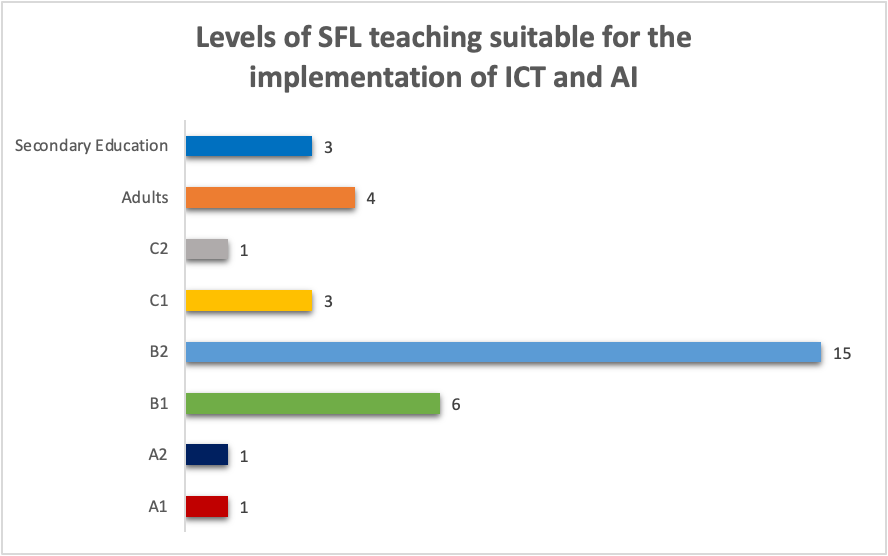
\includegraphics[width=\linewidth]{Images/image1.png}
    \caption{Results for C1.}
    \label{fig-1}
    \source{Own elaboration.}
    \end{minipage}
\end{figure}

\begin{figure}[h!]
    \centering
    \begin{minipage}{0.90\linewidth}
    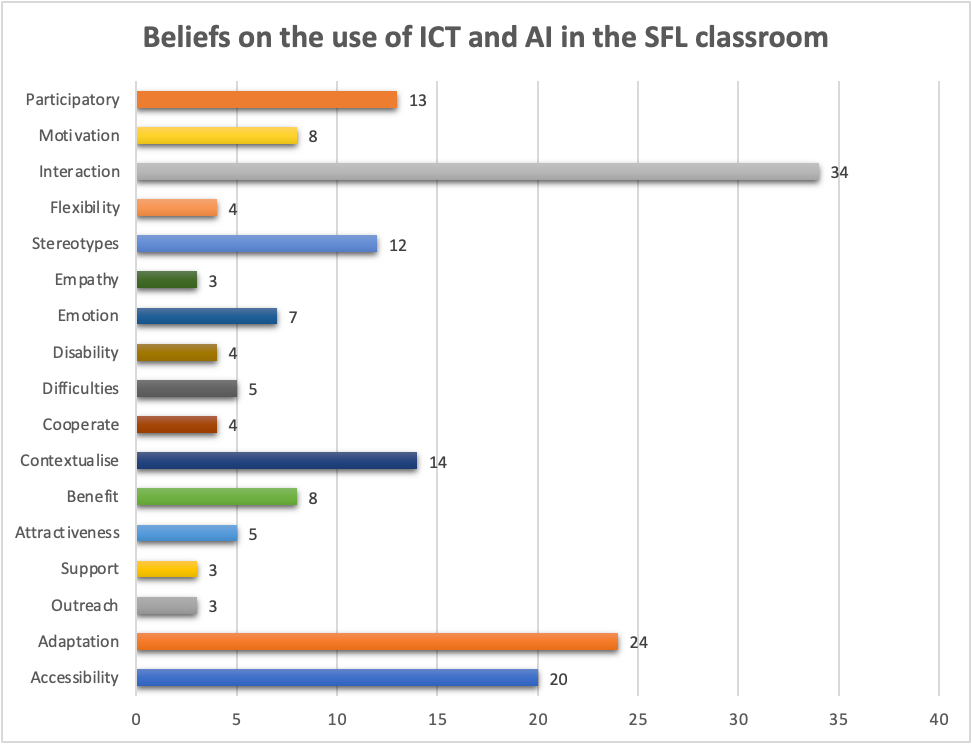
\includegraphics[width=\linewidth]{Images/FIGURA2.png}
    \caption{Results for C2.}
    \label{fig-2}
    \source{Own elaboration.}
    \end{minipage}
\end{figure}

\begin{figure}[h!]
    \centering
    \begin{minipage}{0.90\linewidth}
    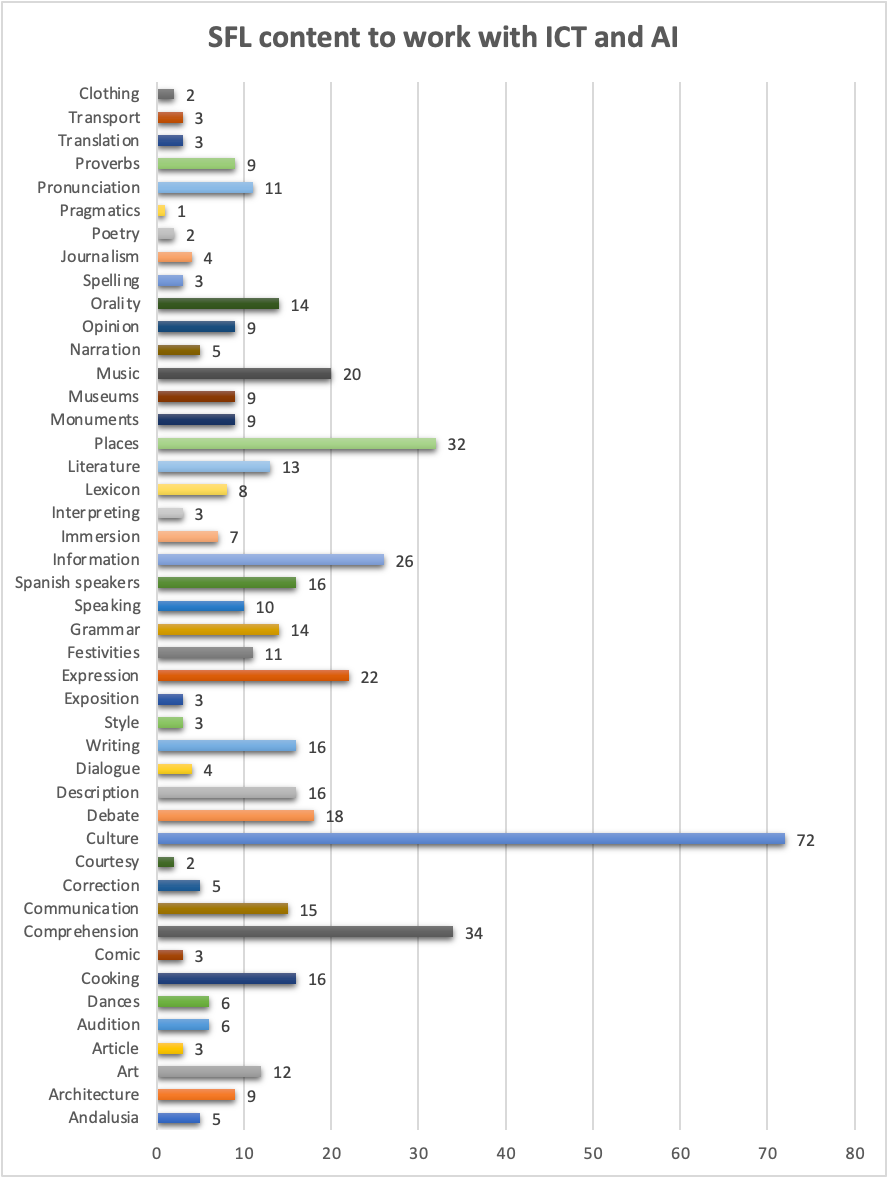
\includegraphics[width=\linewidth]{Images/FIGURA3.png}
    \caption{Results for C3.}
    \label{fig-3}
    \source{Own elaboration.}
    \end{minipage}
\end{figure}

\begin{figure}[h!]
    \centering
    \begin{minipage}{0.90\linewidth}
    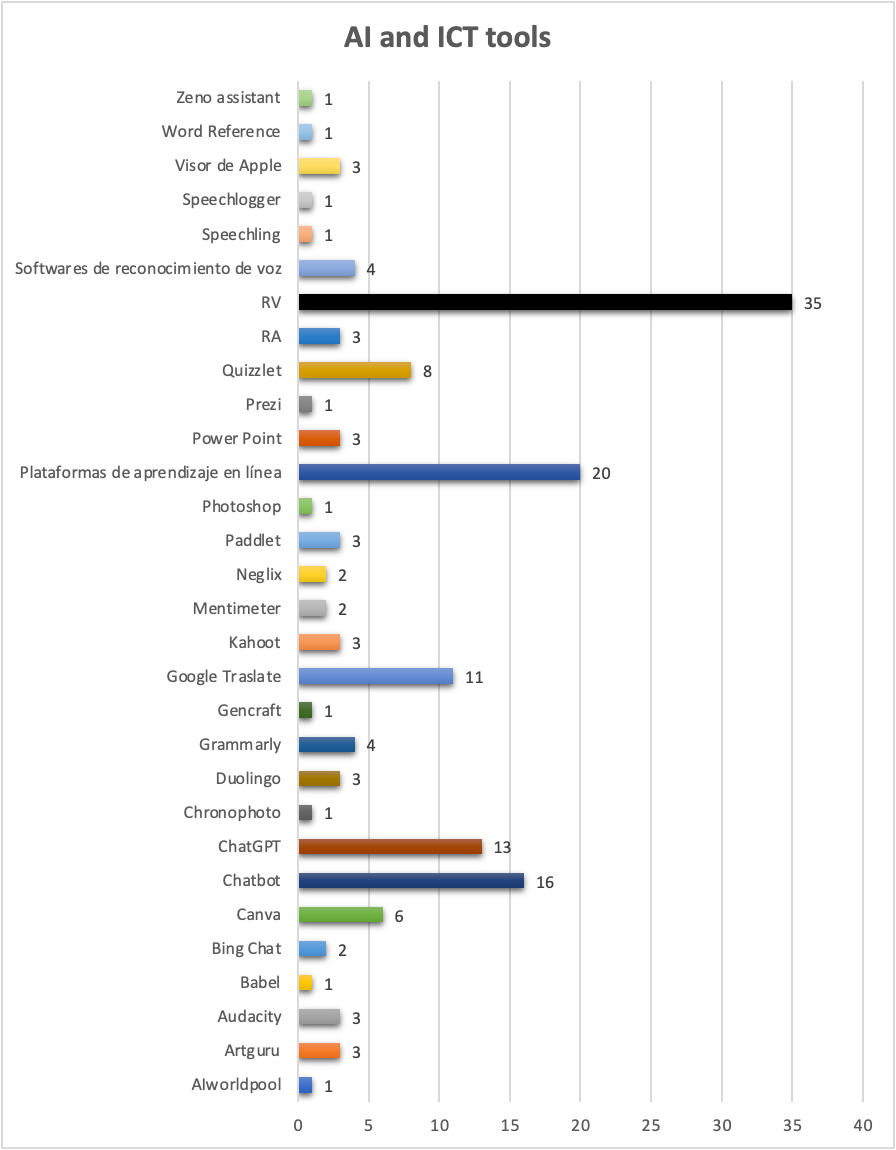
\includegraphics[width=\linewidth]{Images/image4.png}
    \caption{Results for C4.}
    \label{fig-4}
    \source{Own elaboration.}
    \end{minipage}
\end{figure}


\section{Discussion}
\subsection{C1: Educational levels of SFL teaching and the implementation of ICT and AI}
As demonstrated in the initial figure (see Figure \ref{fig-1}), B2 is the most prevalent level with 30 mentions. When augmenting this figure with the number of mentions of B1, it can be expeditiously concluded that the intermediate levels of SFL (B1 and B2) are regarded by the students to be the most suitable for the implementation of ICT and AI. In the initial intervention of the forum (I1), the learner posits that the utilisation of this particular resource is especially pertinent at the B2 level, as it facilitates the exploration and understanding of Spanish-speaking culture and allows the strengthening of language skills in a significant way. In I12, also in relation to level B2, one learner argues that at this stage, learners have developed the linguistic knowledge necessary to communicate in basic aspects of everyday life and therefore at this more advanced level, they need the knowledge of culture that is easily acquired through ICT and AI (I12). Furthermore, four learners (I16, I35, I46 and I50) provide a similar explanation concerning the use of these resources at advanced levels C1 and C2, citing analogous reasons.

One learner (I42) has expressed a divergent opinion, asserting that the utilisation of ICT and AI would be more effectively employed in the preliminary levels (A1 and A2). This assertion is based on the premise that, at these nascent stages, learners require the acquisition of vocabulary pertaining to the most proximate physical environment. The employment of these technologies has the capacity to facilitate the recreation of everyday life.

Finally, a significant group of students, ten in number, initiated a debate on the potential differences in the use of these technologies with students of different ages (I14, I28, I31, I32, I36, I40, I41, I44, I47, I48). While the majority of students generally consider that the use of these tools is more effective with adults, I36 advocates for their implementation from Secondary Education onwards, given that adolescents have regular access to electronic devices and are familiar with their use.

\subsection{C2: Beliefs on the use of ICT and AI in the SFL classroom}

In general terms, the implementation of ICT and AI in the SFL classroom is viewed favourably by students. For instance, I12 states that the integration of artificial intelligence (AI) in this context can also be very beneficial for personalising learning and providing more adaptive and efficient experiences. Indeed, the lexical family relating to the benefits of using these technologies is reiterated up to eight times. The predominant reasons cited by students for the integration of these technologies in terms of sociocultural content are the enhanced accessibility to diverse content (reiterated up to 20 times) and their capacity for adaptation to students' needs (an argument emphasised up to 24 times). These observations align with the findings reported by \textcite{briceno-nunez2024, munoz-basols2024, intria2023}.

The participants place particular emphasis on the educational opportunities that these types of software offer to people with 'disabilities' (lexical family repeated up to four times). At this point, it seems pertinent to recall the statements of \textcite[p. 57]{clementi2024}:

\begin{quote}
El enfoque convencional, que trata a todos los estudiantes como si tuvieran las mismas necesidades educativas, conduce a la creación de programas y objetivos uniformes, así como al desarrollo y elaboración de materiales didácticos estandarizados. Esta práctica, claramente no inclusiva, impide el logro de los objetivos educativos para aquellos que no se ajustan a la norma [...].
En este contexto complejo, la adopción de la Inteligencia Artificial (IA) y la Realidad Aumentada (RA) en la educación lingüística representa un avance hacia métodos didácticos innovadores e inclusivos.
\newline
[The conventional approach, which treats all students as having the same educational needs, leads to the creation of uniform curricula and objectives, and the development and production of standardised learning materials. This clearly non-inclusive practice prevents the achievement of educational goals for those who do not conform to the norm [...].
In this complex context, the use of Artificial Intelligence (AI) and Augmented Reality (AR) in language education represents a step towards innovative and inclusive teaching methods].
\end{quote}

Also mentioned are the increased opportunities for communicative 'interaction' which helps to anchor learning, this being the most represented lexical family with up to 34 repetitions; as well as up to 14 times its benefits in terms of contextualisation (I16 highlights that it provides a rich and authentic context which facilitates language acquisition and promotes a deeper understanding of the language) and the opportunity these technologies offer to turn the SFL classroom into a participatory space (I21 notes that the use of technological tools and AI in the classroom facilitates access to diverse information and promotes active participation), highlighting the opportunities their use offers in the implementation and development of new methodologies in SFL \cite{ayala2023}. Finally, the ``attractiveness" of these tools and the ``flexibility" \cite{moreno-padilla2019, roman2024} they offer are also representative arguments in their favour.

However, some teachers adopt a more cautious stance, highlighting potential disadvantages associated with the use of these resources. For instance, when it comes to learning cultural content in the SFL classroom, the risk of imparting a stereotyped view of reality to students is emphasised up to 12 times. In relation to the utilisation of AI, I63 asserts that these software programs frequently result in the generation of images full of stereotypes, and that, moreover, the AI can be mistaken in its depiction of reality. This resonates with Sandoval's \citeyear{sandoval2024} cautions concerning the biases introduced in the language models of various generative artificial intelligences. I66 is particularly illustrative in this respect, noting that students need to be educated to distinguish between stereotypes and true representations of people living in a country or in specific geographical areas.

Finally, six students have expressed concerns regarding the potential suppression of the emotional aspect that may be associated with the implementation of these technologies, particularly AI. Consequently, these students regard the teacher as an indispensable element in the teaching and learning process. This concern is shared by a considerable sector of the scientific community \cite{martin-marchante2022, canales2024, rodriguez2024, sandoval2024}. I70 asserts that AI is not a substitute for human and empathic interaction and that ``no podría adaptarse a las necesidades especiales de cada alumno y mucho menos proporcionar el mismo apoyo emocional y motivacional que una figura humana [it could not adapt to the special needs of each student, much less provide the same emotional and motivational support as a human figure]". I71 concludes that:

\begin{quote}
    La labor del profesor va más allá de simplemente impartir conocimientos; también implica comprender y apoyar a los estudiantes en su desarrollo integral. La inteligencia emocional desempeña un papel crucial en este proceso, ya que permite al profesor percibir las necesidades y circunstancias individuales de cada alumno, proporcionando una guía y apoyo personalizados que difícilmente puede ser replicado por la inteligencia artificial. Por lo tanto, el contacto humano en la educación sigue siendo fundamental y es poco probable que la inteligencia artificial pueda superarlo en este aspecto, ya que la verdadera misión del docente va más allá de la simple transmisión de información.
    \newline
    [The role of the teacher extends beyond the mere transmission of knowledge; it encompasses the responsibility to comprehend and nurture students' holistic development. Emotional intelligence is a pivotal component of this process, as it enables the teacher to discern the unique needs and contexts of each student, thereby providing bespoke guidance and support that is difficult to replicate with artificial intelligence. Consequently, human interaction in education remains indispensable, and it is implausible that artificial intelligence can surpass it in this domain, as the true mission of the teacher transcends the mere transmission of information].
\end{quote}

\textcite{intria2023} thus posit that the mere use of these platforms does not guarantee effective teaching. Unfortunately, not all students participated in this debate from the outset, as evidenced by the number of interventions, which commenced almost at the end of the forum.

\subsection{C3: SFL content for working with ICT and AI}
When it comes to selecting SFL content for the implementation of ICT and AI in the classroom, students opted for those related to ‘culture’ (lexical family represented on up to 72 occasions). Thus, among the most frequently repeated cultural contents are gastronomy, with the lexical family relating to ‘cuisine’ being mentioned up to 16 times; traditional festivals, with up to 11 repetitions; emblematic monuments and geographical places, with 9 and 32 repetitions respectively; museums, whose lexical family is also repeated 9 times; music, mentioned up to 20 times; and finally, proverbs or sayings, which are mentioned 9 times. As demonstrated \cite{cervantes2006}, the majority of these contents are found within the domain of socio-cultural knowledge and behaviour, with a smaller proportion falling under the category of cultural references. It is therefore noteworthy that learners have excluded those related to intercultural skills and attitudes, particularly in light of the assertion that the primary rationale for incorporating ICT and AI in the SFL classroom is to enhance communicative interaction. This exclusion may be attributed to several factors: learners may perceive such communicative interaction as 'unreal' to be provided by a technological tool; or they may find it more difficult to work on the contents of the inventory of intercultural skills and attitudes and, therefore, avoid such contents or understand that they should be dealt with directly by the teacher.

In addition to the cultural dimension, some learners emphasise the advantages that these technologies offer in the classroom, particularly in relation to ‘grammar’ (14 instances), ‘vocabulary’ (6 instances), ‘linguistic correctness’ (5 instances), ‘spelling’ (3 instances), ‘pronunciation’ (11 instances), and ‘pragmatics’ (1 instance). Furthermore, several learners insist on the role that these technologies could play in the work on macro language skills:  the term 'writing' is mentioned 16 times; 'speaking' or 'orality', up to 24 times in total; and 'reading', up to 14 times. For example, I32 points that two suitable tools for working on literature in the classroom are augmented reality and AI.

Finally, a multitude of interventions allude to the oeuvre of specific discursive genres and particular textual sequences. Among the discursive genres cited, 'debate' is notable, with 18 repetitions, as I27 observes, ICT promoting the organisation of online debates. The most recurrent textual sequence is 'description', intimately associated with the contextualisation capacity proffered by ICT and AI, mentioned 16 times. Finally, I34 is worthy of note, as it refers to the potential creating images through precise descriptions' in connection with generative software.

\subsection{C4: AI and ICT tools}
The objective of this section was to investigate the ICT and AI tools that students are familiar with and utilise, with a view to their implementation in the SFL classroom context. As illustrated in Figure \ref{fig-4}, Virtual Reality (VR), in its various forms, namely immersive, non-immersive, and semi- immersive, emerges as the most frequently cited tool by students, with up to 32 repetitions. I48 states that virtual reality provides the opportunity to transport students to remote locations without leaving the classroom, while I56 mentions that virtual reality platforms allow students to immerse themselves in virtual environments that recreate historical and cultural places.

Secondly, if we add references to ChatGPT and chatbots in general, we find automated chats, especially useful for the acquisition of communicative fluency \cite{guano2023, lucana2023, de-almeida-ferreira2024}. Thus, in I71 it is noted that specialised chatbots can be used to interact with students and improve their communication skills, as if they were teachers \cite{moreno-padilla2019}. Other learners point out that these types of applications are also particularly useful when searching for information, as they can talk to students about specific cultural topics (I23).

Thirdly, online learning platforms are mentioned up to 20 times, as they allow fluency practice and receive feedback on their accuracy without the teacher having to be present (I34). The same intervention refers to voice recognition platforms such as Speechlogger, Speechling or Babel, as well as one of the best known by learners, Duolingo, mentioned in two other interventions (I36 and I60). These software programmes are positioned as a hybrid of generative AI and ICT for education, with a special design for language learning purposes \cite{coello-munoz2023}.

Finally, it is striking how the three most frequently mentioned tools belong to the field of AI, with the use of ICT barely mentioned by pupils. Kahoot is mentioned on three occasions; Paddlet, on another three occasions; Photoshop, only once; PowerPoint, again on three occasions; Prezi, only once; and WordReference, also only once. Quizzlet is the most frequently mentioned non-AI tool, with eight repetitions. This does not necessarily imply that students disregard ICT in favour of AI; rather, it may be indicative of their familiarity with ICT, which has been extensively promoted in educational settings over the past few decades \cite{balart2018tic}. In contrast, the integration of AI in the classroom is a relatively recent development.

\section{Conclusions}
The findings of our investigation into the beliefs of prospective teachers enrolled in the Master's Degree Programme in Spanish Language and Literature: research and applications reveal a multifaceted perspective on the utilisation and integration of Information and Communication Technologies (ICT) and Artificial Intelligence (AI). On the one hand, it is evident that participants recognise and value the positive nature of technology during the teaching-learning process, especially at intermediate levels. Participants identified several advantages of technology in the classroom, including its accessibility, the opportunity for personalisation of learning, and the possibilities for communicative interaction. However, they also expressed concerns about the potential distractions that technology might introduce in the classroom, particularly for learners of SFL, and the potential inequalities that access to these tools might entail. This perspective, arguably overly optimistic, signifies an openness to pedagogical innovation and a readiness to integrate these tools into future teaching practices, a prerequisite for adapting Spanish language teaching in the digital age.

However, it is equally important to consider the potential negative consequences of technological integration, such as the suppression of emotions and human interaction. This concern aligns with the research conducted by \textcite{canales2024} and \textcite{sandoval2024}, emphasising the significance that teachers in SFL training attribute to socioemotional aspects in the learning and integral development of students. It also validates the role of the teacher as a facilitator in the teaching and learning process \cite{martin-marchante2022, rodriguez2024}. This is a valid concern for the participants, as a strong commitment to the implementation of AI, particularly conversational assistants in the teaching role \cite{moreno-padilla2019}, could result in job losses.

Regarding to the interrelationship between the contents and the technological tools, as would be anticipated in view of the subject in which the research was conducted, the pupils underscore the importance of engaging with cultural references and socio-cultural knowledge and behaviour \cite{cervantes2006}. However, the omission of an inventory relating to intercultural skills and attitudes highlights the necessity of instilling in students the understanding that engagement with these subjects is imperative for cultivating intercultural competence within the context of the SFL classroom.

Finally, with regard to the software most frequently used by the participants, virtual reality (VR) and chatbots are noteworthy \cite{guano2023, lucana2023, de-almeida-ferreira2024}. This does not imply that students' use of more conventional ICT tools is being neglected, as their responses may be attributable to the appeal of novelty.

In conclusion, the findings emphasise the necessity to reconcile the integration of ICT and AI in the process of acquiring SFL. In this context, teacher training should not only focus on developing technical competences, but also on the acquisition of strategies aimed at maintaining and fostering emotional connection with learners, while developing their linguistic and intercultural competence. Future research should explore how digital and AI models can be implemented in a way that complements rather than replaces communication for meaningful learning and the development of educational policies that support the responsible use of such technology.

\printbibliography\label{sec-bib}
% if the text is not in Portuguese, it might be necessary to use the code below instead to print the correct ABNT abbreviations [s.n.], [s.l.]
%\begin{portuguese}
%\printbibliography[title={Bibliography}]
%\end{portuguese}


%full list: conceptualization,datacuration,formalanalysis,funding,investigation,methodology,projadm,resources,software,supervision,validation,visualization,writing,review
\begin{contributors}[sec-contributors]
\authorcontribution{María García Fernández}[conceptualization,methodology,validation,formalanalysis,investigation,resources,datacuration,writing,review,visualization,supervision,projadm,funding]
\authorcontribution{Rocío Jodar Jurado}[conceptualization,methodology,validation,formalanalysis,investigation,resources,datacuration,writing,review,visualization,supervision,projadm,funding]
\authorcontribution{Carmen María Sánchez Morillas}[conceptualization,methodology,validation,formalanalysis,investigation,resources,datacuration,writing,review,visualization,supervision,projadm,funding]
\end{contributors}

\end{document}

